\documentclass[journal,12pt,twocolumn]{IEEEtran}
\makeatletter
\@addtoreset{figure}{problem}
\makeatother
\usepackage{setspace}
\usepackage{gensymb}
\usepackage{xcolor}
\usepackage{caption}
%\usepackage{multirow}
%\usepackage{multicolumn}
%\usepackage{subcaption}
%\doublespacing
\singlespacing
\usepackage{amsmath}
\usepackage{multicol}
\usepackage{enumerate}
\usepackage{amssymb}
\usepackage{iithtlc}
%\usepackage{graphicx}
\usepackage{newfloat}
%\usepackage{syntax}
\usepackage{listings}
\usepackage{color}
\usepackage{tikz}
%\usepackage{tikz}
\usepackage{tkz-euclide}
\usetkzobj{all}
\usepackage[american]{circuitikz}
\usetikzlibrary{shapes,arrows}



%\usepackage{graphicx}
%\usepackage{amssymb}
%\usepackage{relsize}
%\usepackage[cmex10]{amsmath}
%\usepackage{mathtools}
%\usepackage{amsthm}
%\interdisplaylinepenalty=2500
%\savesymbol{iint}
%\usepackage{txfonts}
%\restoresymbol{TXF}{iint}
%\usepackage{wasysym}
\usepackage{amsthm}
\usepackage{mathrsfs}
\usepackage{txfonts}
\usepackage{stfloats}
\usepackage{cite}
\usepackage{cases}
\usepackage{mathtools}
\usepackage{caption}
\usepackage{enumerate}	
\usepackage{enumitem}
\usepackage{amsmath}
%\usepackage{xtab}
\usepackage{longtable}
\usepackage{multirow}
%\usepackage{algorithm}
%\usepackage{algpseudocode}
\usepackage{enumitem}
\usepackage{mathtools}

%\usepackage[framemethod=tikz]{mdframed}
\usepackage{listings}
\usepackage{listings}
    %\usepackage[latin1]{inputenc}                                 %%
    \usepackage{color}                                            %%
    \usepackage{array}                                            %%
    \usepackage{longtable}                                        %%
    \usepackage{calc}                                             %%
    \usepackage{multirow}                                         %%
    \usepackage{hhline}                                           %%
    \usepackage{ifthen}                                           %%
  %optionally (for landscape tables embedded in another document): %%
    \usepackage{lscape}     



%\usepackage{stmaryrd}


%\usepackage{wasysym}
%\newcounter{MYtempeqncnt}
\DeclareMathOperator*{\Res}{Res}
%\renewcommand{\baselinestretch}{2}
\renewcommand\thesection{\arabic{section}}
\renewcommand\thesubsection{\thesection.\arabic{subsection}}
\renewcommand\thesubsubsection{\thesubsection.\arabic{subsubsection}}

\renewcommand\thesectiondis{\arabic{section}}
\renewcommand\thesubsectiondis{\thesectiondis.\arabic{subsection}}
\renewcommand\thesubsubsectiondis{\thesubsectiondis.\arabic{subsubsection}}

% correct bad hyphenation here
\hyphenation{op-tical net-works semi-conduc-tor}

%\lstset{
%language=C,
%frame=single, 
%breaklines=true
%}

%\lstset{
	%%basicstyle=\small\ttfamily\bfseries,
	%%numberstyle=\small\ttfamily,
	%language=Octave,
	%backgroundcolor=\color{white},
	%%frame=single,
	%%keywordstyle=\bfseries,
	%%breaklines=true,
	%%showstringspaces=false,
	%%xleftmargin=-10mm,
	%%aboveskip=-1mm,
	%%belowskip=0mm
%}

%\surroundwithmdframed[width=\columnwidth]{lstlisting}
\def\inputGnumericTable{}                                 %%
\lstset{
language=C,
frame=single, 
breaklines=true
}
 

\begin{document}
%
\tikzstyle{block} = [rectangle, draw,
    text width=4em, text centered, minimum height=3em]
\tikzstyle{sum} = [draw, circle, node distance=3cm]
\tikzstyle{input} = [coordinate]
\tikzstyle{output} = [coordinate]
\tikzstyle{pinstyle} = [pin edge={to-,thin,black}]

\theoremstyle{definition}
\newtheorem{theorem}{Theorem}[section]
\newtheorem{problem}{Problem}
\newtheorem{proposition}{Proposition}[section]
\newtheorem{lemma}{Lemma}[section]
\newtheorem{corollary}[theorem]{Corollary}
\newtheorem{example}{Example}[section]
\newtheorem{definition}{Definition}[section]
%\newtheorem{algorithm}{Algorithm}[section]
%\newtheorem{cor}{Corollary}
\newcommand{\BEQA}{\begin{eqnarray}}
\newcommand{\EEQA}{\end{eqnarray}}
\newcommand{\define}{\stackrel{\triangle}{=}}

\bibliographystyle{IEEEtran}
%\bibliographystyle{ieeetr}

\providecommand{\nCr}[2]{\,^{#1}C_{#2}} % nCr
\providecommand{\nPr}[2]{\,^{#1}P_{#2}} % nPr
\providecommand{\mbf}{\mathbf}
\providecommand{\pr}[1]{\ensuremath{\Pr\left(#1\right)}}
\providecommand{\qfunc}[1]{\ensuremath{Q\left(#1\right)}}
\providecommand{\sbrak}[1]{\ensuremath{{}\left[#1\right]}}
\providecommand{\lsbrak}[1]{\ensuremath{{}\left[#1\right.}}
\providecommand{\rsbrak}[1]{\ensuremath{{}\left.#1\right]}}
\providecommand{\brak}[1]{\ensuremath{\left(#1\right)}}
\providecommand{\lbrak}[1]{\ensuremath{\left(#1\right.}}
\providecommand{\rbrak}[1]{\ensuremath{\left.#1\right)}}
\providecommand{\cbrak}[1]{\ensuremath{\left\{#1\right\}}}
\providecommand{\lcbrak}[1]{\ensuremath{\left\{#1\right.}}
\providecommand{\rcbrak}[1]{\ensuremath{\left.#1\right\}}}
\theoremstyle{remark}
\newtheorem{rem}{Remark}
\newcommand{\sgn}{\mathop{\mathrm{sgn}}}
\providecommand{\abs}[1]{\left\vert#1\right\vert}
\providecommand{\res}[1]{\Res\displaylimits_{#1}} 
\providecommand{\norm}[1]{\lVert#1\rVert}
\providecommand{\mtx}[1]{\mathbf{#1}}
\providecommand{\mean}[1]{E\left[ #1 \right]}
\providecommand{\fourier}{\overset{\mathcal{F}}{ \rightleftharpoons}}
%\providecommand{\hilbert}{\overset{\mathcal{H}}{ \rightleftharpoons}}
\providecommand{\system}{\overset{\mathcal{H}}{ \longleftrightarrow}}
	%\newcommand{\solution}[2]{\textbf{Solution:}{#1}}
\newcommand{\solution}{\noindent \textbf{Solution: }}
\providecommand{\dec}[2]{\ensuremath{\overset{#1}{\underset{#2}{\gtrless}}}}
\DeclarePairedDelimiter{\ceil}{\lceil}{\rceil}
%\numberwithin{equation}{subsection}
\numberwithin{equation}{problem}
%\numberwithin{problem}{subsection}
%\numberwithin{definition}{subsection}
%\makeatletter
%\@addtoreset{figure}{problem}
%\makeatother

%\let\StandardTheFigure\thefigure
%\renewcommand{\thefigure}{\theproblem.\arabic{figure}}
%\renewcommand{\thefigure}{\theproblem}


%\numberwithin{figure}{section}

%\numberwithin{equation}{subsection}
%\numberwithin{equation}{section}
\numberwithin{equation}{problem}
%\numberwithin{problem}{subsection}
\numberwithin{problem}{section}
%%\numberwithin{definition}{subsection}
%\makeatletter
%\@addtoreset{figure}{problem}
%\makeatother
%\makeatletter
%\@addtoreset{table}{problem}
%\makeatother

%\let\StandardTheFigure\thefigure
%\let\StandardTheTable\thetable
%\numberwithin{table}{section}
%%\renewcommand{\thefigure}{\theproblem.\arabic{figure}}
%\renewcommand{\thefigure}{\theproblem}

%%\numberwithin{figure}{section}

%%\numberwithin{figure}{subsection}



\def\putbox#1#2#3{\makebox[0in][l]{\makebox[#1][l]{}\raisebox{\baselineskip}[0in][0in]{\raisebox{#2}[0in][0in]{#3}}}}
     \def\rightbox#1{\makebox[0in][r]{#1}}
     \def\centbox#1{\makebox[0in]{#1}}
     \def\topbox#1{\raisebox{-\baselineskip}[0in][0in]{#1}}
     \def\midbox#1{\raisebox{-0.5\baselineskip}[0in][0in]{#1}}

\vspace{3cm}

\title{ 
	\logo{
DC-AC Converter
	}
}

\author{B Swaroop Reddy and  G V V Sharma$^{*}$% <-this % stops a space
	\thanks{*The author is with the Department
		of Electrical Engineering, Indian Institute of Technology, Hyderabad
		502285 India e-mail:  gadepall@iith.ac.in. All content in this manual is released under GNU GPL.  Free and open source.}
	
}	

\maketitle

\tableofcontents
\bigskip

\begin{abstract}
	
	This manual provides the design of a DC-AC Converter.
	
\end{abstract}

%\section{Buck Converter}
\section{Components}
\begin{table}[!h]
\centering
\input{./figs/components.tex}
\caption{}
\label{table:components}
\end{table}
\section{Circuit Operation}
The DC-AC converter Block diagram and circuit are shown in Fig. \ref{fig1} and Fig. \ref{fig2}
\begin{figure}[!h]
\centering
\resizebox {\columnwidth} {!} {
\begin{circuitikz}
      \draw (0,-4)
    to[V,v<=$V_{s}$] (0,4)
     
    %to [L=$L$] (2,4)
    to [short] (4,4)
    to [short] (4,3)
    (4,2.5) node[nigfete] (nmos) {}
    (nmos.S) to (4,-1)
    (nmos.G) to (3,2)
   %to [short] (3.5,2.5)
    (2,2.5) node[block]{{\textbf{GATE DRIVER}}}
    (2.5,1.9) to [short] (2.5,1.5) 
    to [short] (4,1.5)
    (4,-1.5) node[nigfete] (nmos) {}
    (nmos.S) to (4,-4)
    to [short] (0,-4)
    (nmos.G) to (3,-1.5)
    (2,-1.5) node[block]{{\textbf{GATE DRIVER}}}
    (4,4) to [short] (8,4)
    to [short] (8,3)
    (8,2.5) node[nigfete] (nmos) {}
    (nmos.S) to (8,-1)
    (nmos.G) to (7,2)
   %to [short] (3.5,2.5)
    (6,2.5) node[block]{{\textbf{GATE DRIVER}}}
    (6.5,1.9) to [short] (6.5,1.5) 
    to [short] (8,1.5)
    (8,-1.5) node[nigfete] (nmos) {}
    (nmos.S) to (8,-4)
    to [short] (0,-4)
    (nmos.G) to (7,-1.5)
    (6,-1.5) node[block]{{\textbf{GATE DRIVER}}}
    (4,0) to [short] (5,0)
    (5.7,0) node[rectangle, draw,
    text width=3em, text centered, minimum   
              height=1.5em]{{\textbf{Load}}}
    (6.4,0) to [short] (8,0)
    
    %to[V,v<=$V_{s}$] (0,0)
    %to [short] (3.8,0)
    %to [short] (3.8,0.2)
    %(3.8,0) .. controls (4,0) .. (4.2,0)
    %to [short] (4.2,0.2)
    %to [short] (4.2,0)
    %to [short] (5,0)
    %(5.7,0) node[rectangle, draw,
    %text width=3em, text centered, minimum   
     %         height=1.5em]{{\textbf{Load}}}
    %(6.5,0)to [short] (7.5,0)
    %to [short] (7.5,0.7)
    %to [short] (4,0.7)
    %(2.5,-2.1) to [short] (2.5,-2.5)
    %to [short] (4,-2.5)
    %(4,4) to [D,l=$D$] (7,4)
    %to [short] (8.5,4)
    %to [R=$R$] (8.5,0)
     %to[short] (0,0)
    %(7,4) to [C=$C$] (7,0)
   ;  
    \end{circuitikz}
   
}
\caption{DC-AC converter} 
\label{fig1}
\end{figure}
\begin{figure}[!h]
\centering
\resizebox {\columnwidth} {!} {
\begin{tikzpicture}

\node[draw,text width=3em] at (0,15) {DC Source};
\node[draw,text width=5em] at (10,13) {MOSFET 1};
\node[draw,text width=5em] at (15,13) {MOSFET 2};
\node[draw,text width=5em] at (10,11) {Gate Driver};
\node[draw,text width=5em] at (15,11) {Gate Driver };
\node[draw,text width=4em] at (3,9) {Arduino};
\node[draw,text width=8em,align=center] at (7,9) {Dead-Band Circuit};
\node[draw,text width=5em] at (10,6) {Gate Driver};
\node[draw,text width=5em] at (15,6) {Gate Driver};
\node[draw,text width=5em] at (10,4) {MOSFET 3};
\node[draw,text width=5em] at (15,4) {MOSFET 4};
\node[draw,text width=3em] at (14,0) {LPF};
\draw (0.8,15) -- (14.8,15);
\draw (14.8,15) -- (14.8,13.3);
\draw (10,15) -- (10,13.3);
\draw (10,12.7) -- (10,11.3);
\draw (14.8,12.7) -- (14.8,11.3);
\draw  (10,10.7)--(10,9.19);
\draw (10,8.9)--(10,6.3);
\draw (10,5.7)--(10,4.3);
\draw (14.8,5.7)--(14.8,4.3);
\draw (4,9)--(5.2,9);
\draw (1,15)--(1,3);
\draw (1,3)--(14.8,3);
\draw (12,13)--(12,2);
\draw (11.2,13)--(12,13);
\draw (16.2,13)--(16.8,13);
\draw (8.8,9.2)--(14.8,9.2);
\draw (8.8,8.9)--(13.5,8.9);
\draw(13.5,8.9)--(13.5,11);
\draw(13.5,11)--(13.8,11);
\draw (14.8,9.2)--(14.8,6.3);
\draw (14.8,3)--(14.8,3.7);
\draw (16.8,13)--(16.8,2);
\draw (13.6,2)--(12,2);
\draw (14,2--(1,1);
\draw (14,2)--(16.8,2);
\draw(13.6,0.3)--(13.6,2);
\draw(14,0.3)--(14,2);
\draw(16.2,4)--(16.8,4);
\draw(11.2,4)--(12,4);
\draw(14.8,0.1)--(16,0.1);
%\draw(14.8,-0.14)--(16,-0.14);
\draw(10,3.7)--(10,3);
\node[below left= 1mm of {(10,14)}] {$D$};
\node[below left= 1mm of {(14.8,14)}] {$D$};
\node[below left= 1mm of {(10,12)}] {$G$};
\node[below left= 1mm of {(14.8,12)}] {$G$};
\node[below left= 1mm of {(12,13.5)}] {$S$};
\node[below left= 1mm of {(17,13.5)}] {$S$};
\node[below left= 1mm of {(10.6,5)}] {$G$};
\node[below left= 1mm of {(15.4,5)}] {$G$};
\node[below left= 1mm of {(12,4.7)}] {$D$};
\node[below left= 1mm of {(16.8,4.7)}] {$D$};
\node[below left= 1mm of {(10.6,3.8)}] {$S$};
\node[below left= 1mm of {(15.4,3.8)}] {$S$};
\node[below left= 1mm of {(16.8,0.4)}] {$V_{ac}$};
\node[below left= 1mm of {(9.5,9.7)}] {$1$};
\node[below left= 1mm of {(9.5,9)}] {$2$};
\node[below right= 1mm of {(0.7,15.28)}] {$\bullet$};
\node[below right= 1mm of {(9.7,15.28)}] {$\bullet$};
%\node[below right= 1mm of {(11.7,4.3)}] {$\bullet$};
\node[below right= 1mm of {16.5,4.3)}] {$\bullet$};



\end{tikzpicture}

}
\caption{DC-AC converter Block-diagram} 
\label{fig2}
\end{figure}

\begin{problem}
Generate 4 dc sources of +12 V and -5 V each using the voltage regulator circuit as shown in the Fig.\ref{fig3}  
  \end{problem}

\begin{figure}[!h]
\centering
\resizebox {\columnwidth} {!} {
\input{./figs/regulator_circuit.tex}
}
\caption{Voltage-Regulator Circuit} 
\label{fig3}
\end{figure}
\begin{problem}
Program the arduino to generate a square wave with {\em Duty Cycle} $D=0.5$ and frequency $f=50 Hz$ and observe the waveform on the oscilloscope. 
\end{problem}
\solution
\lstinputlisting{./codes/square_wave.ino} 
\begin{problem}
Calculate the R and C values for the dead band circuit shown in Fig.\ref{fig4} for the delay of \\ 2.5 $\mu$sec.
\end{problem}
\begin{figure}[!h]
\centering
\resizebox {\columnwidth} {!} {
\input{./figs/dead_band_circuit.tex}
}
\caption{Dead-Band Circuit} 
\label{fig4}
\end{figure}
\solution
\begin{align*}
V_{th}(Logic Gate) &= V_{pulse}(High level) \times (1-e^{-\dfrac{t}{RC}})\\
RC &= 3.82 \times 10^{-6}
\end{align*}
selected  R = 390$\ohm$ and C = 10nF 
\begin{problem}
Connect the $13^{th}$ pin of arduino to the Dead-band circuit and generate the Non-inverted(at 1) and Inverted(at 2) pulses and observe them on the oscilloscope.
\end{problem}
\begin{problem}
Assemble the DC-AC circuit according to Figs. \ref{fig1},\ref{fig2}, \ref{fig5} and Table \ref{table:connections}.
\end{problem}
%\section{Circuit Diagram}
%The circuit diagram is shown in \ref{fig1}
\begin{figure}[!h]
\centering
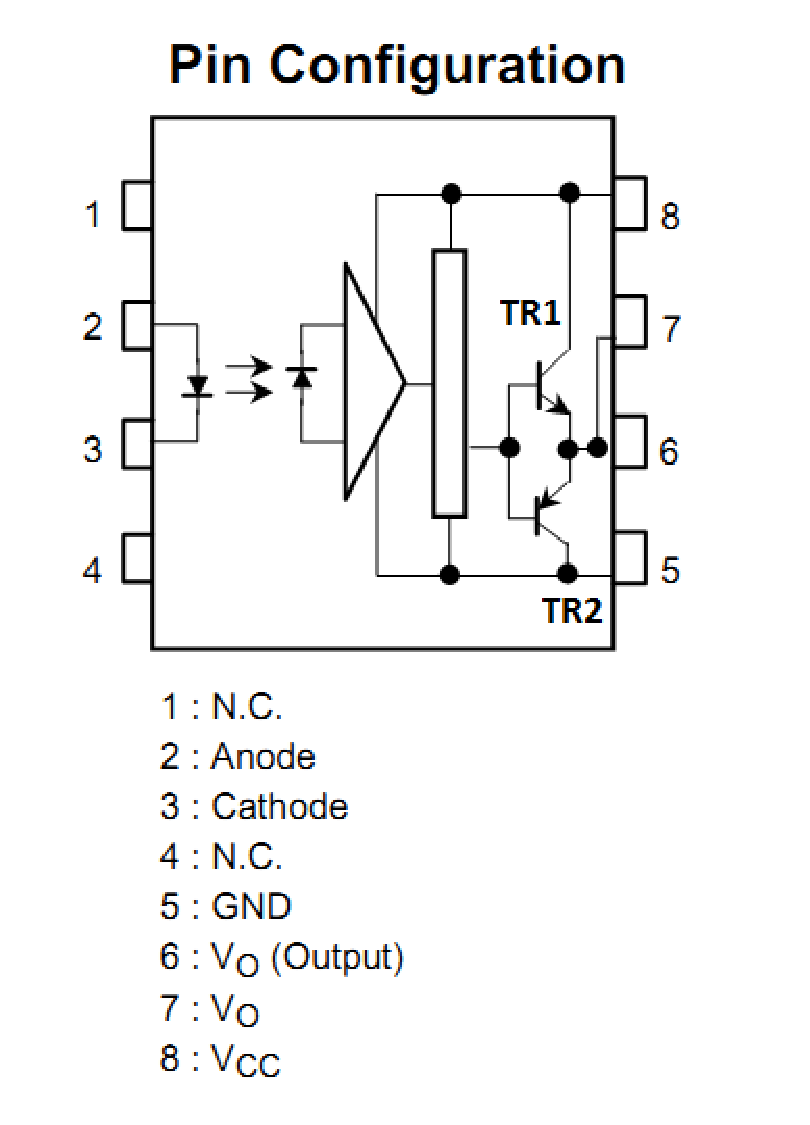
\includegraphics[width=\columnwidth]{./figs/pinout.eps}
\caption{ TLP350}  
\label{fig5}
\end{figure}

%\subsection{\textbf{Gate Driver circuit}}
%The pin description for Opto coupler(TLP350) is shown in fig \ref{fig4}
%Made connections as per the fig \ref{fig2}    
\begin{table}[!h]
\centering
\resizebox {\columnwidth} {!} {
\input{./figs/connections.tex}
}
\caption{Pin Connections} 
\label{table:connections}
\end{table}  

\section{Fourier Series Analysis of DC-AC Converter}
\begin{problem}
Observe the output across the load in Fig. \ref{fig1} on the oscilloscope. What do you observe? \label{prob:problem3.1}
\end{problem}
\begin{problem}
Find the Fourier series expansion for the result in Problem.\ref{prob:problem3.1}.
\end{problem}
\begin{problem}
Design a $4^{th}$ order RC Low pass filter with cut-off frequency 50 Hz and observe the output of the Low pass filter.\label{prob:problem3.3}
\end{problem} 
\begin{problem}
Find the output of the lowpass filter designed in \ref{prob:problem3.3} with input as obtained from the result of \ref{prob:problem3.1}. What do you observe? \label{prob:problem3.4}
\end{problem}
\end{document}
